\documentclass[a4paper]{report}
\usepackage{tikz}
\usepackage{minted}
\usepackage{hyperref}
\usepackage{graphicx}
\usepackage{fontspec}
\usetikzlibrary{shapes.geometric, arrows}
\usemintedstyle{vs}
\graphicspath{ {./images/} }
\setlength{\parindent}{0pt}
\setlength{\parskip}{1em}
\title{A Level Programming Project Report}
\author{Junrong Chen}
\date{\today}

\begin{document}
\maketitle
\tableofcontents
\clearpage
\chapter{Analysis}

\section{Description of the problem}

A Level Computer Science students need to learn many algorithms and data structures during the course. In the final exam, they need to write pseudocode to solve computational questions. Many students find it is hard to achieve a high score on those questions due to the lack of efficient training. The general method used by students to learn and revise for Computer Science is to attempt and self-mark past paper questions. This works well for ordinary questions. However, for the algorithm questions, different students may produce completely different code solutions. This makes their self-marking very unreliable. It is also too much work for the teacher to mark their solutions one by one. So, in the end, students do not know whether they get things right, and teachers do not know how the students perform and how they can help - especially in this lockdown online learning era where no direct contact between teachers and students is possible.

Both the students and the teachers are looking for a more efficient method to learn and practice.

\section{Stakeholders}

There are two types of stakeholders, Computer Science teachers and Computer Science students.

\subsection{Computer Science teachers}

Computer Science teachers find it is difficult to monitor their students' ability to design and implement algorithms, so they cannot provide efficient help to their students. This software allows them to create coding questions and send them to the students. After the students hand their solutions back, the software will automatically mark their answers and provide detailed statistical data with simple visualisations. This helps the teachers saving a lot of time and allows them to help the students better.

(TODO): Find actual stakeholders

\subsection{Computer Science students}

Computer Science students find that they tend to lose mark on the algorithms coding questions, so they want more practice. But unlike ordinary questions, they may take a completely different approach towards the questions comparing to the mark scheme, so they do not know whether they get it correct. Students may also think they have got things right, but actually, they have made some mistakes. The software provides a free practice space that automatically marks their solutions and points out their mistakes in real-time. So the students can learn and revise more efficiently.

(TODO): Find actual stakeholders

\section{Solve by computational methods}

\subsection{Thinking abstractly}

In reality, students use pen and paper to write their code solutions. This can be simplified by a code editor and the students can use the keyboard to type in their code. In this way, no `text scanning' or `handwriting recognization' is needed which makes the designing and programming much easier. The code editor will also provide a better user experience. Features such as syntax highlighting cannot exist on paper but are possible in the abstracted code editor.

In reality, the students' answer is sent to a teacher to mark it against the mark scheme. The teacher needs to read the code line by line and check whether it is correct. This process is simplified into a judger that marks the code against pre-generated test cases, which transforms a problem that originally cannot be solved by computational method into one which is very easy to be solved by a computer while saving time and costs. When creating a new question, instead of creating a mark scheme for marking, the teacher needs to provide test cases with the correct input and expected output. The judger will run the students' submissions with the input and check whether their output matches the expected one.

\subsection{Thinking ahead}

There are two types of input required.

For the teacher, the software requires them to input the question and test cases as a text file. A question editor need to be provided for this purpose.

For the students, the software requires them to input their code solutions to give them feedback. A code editor need to be provided for this purpose.

A relational database is need to store all the input data.

(TODO)

\subsection{Thinking procedurally and decomposition}

The program will be decomposed into several parts.

\begin{itemize}
    \item Code editor
    \item Question editor
    \item Local database
    \item Data analyzer
    \item Judger
    \item GUI
\end{itemize}

(TODO)

\subsection{Thinking concurrently}

When auto judging the solution, many test cases can be executed at the same time to reduce the judging time for large test cases.

(TODO)

\section{Research}

There are many coding training websites on the market, most of them share the similar idea, so I will investigate two of the most popular ones.

\begin{itemize}
    \item LeetCode
    \item Codeforces
\end{itemize}

\subsection{LeetCode}

\href{https://leetcode.com/}{LeetCode} is a platform for interview coding training, many large companies (Google, Facebook, ...) use it as a part of their interview.

LeetCode provides a database containing more than 1000 coding questions.

\subsubsection{Main coding layout}
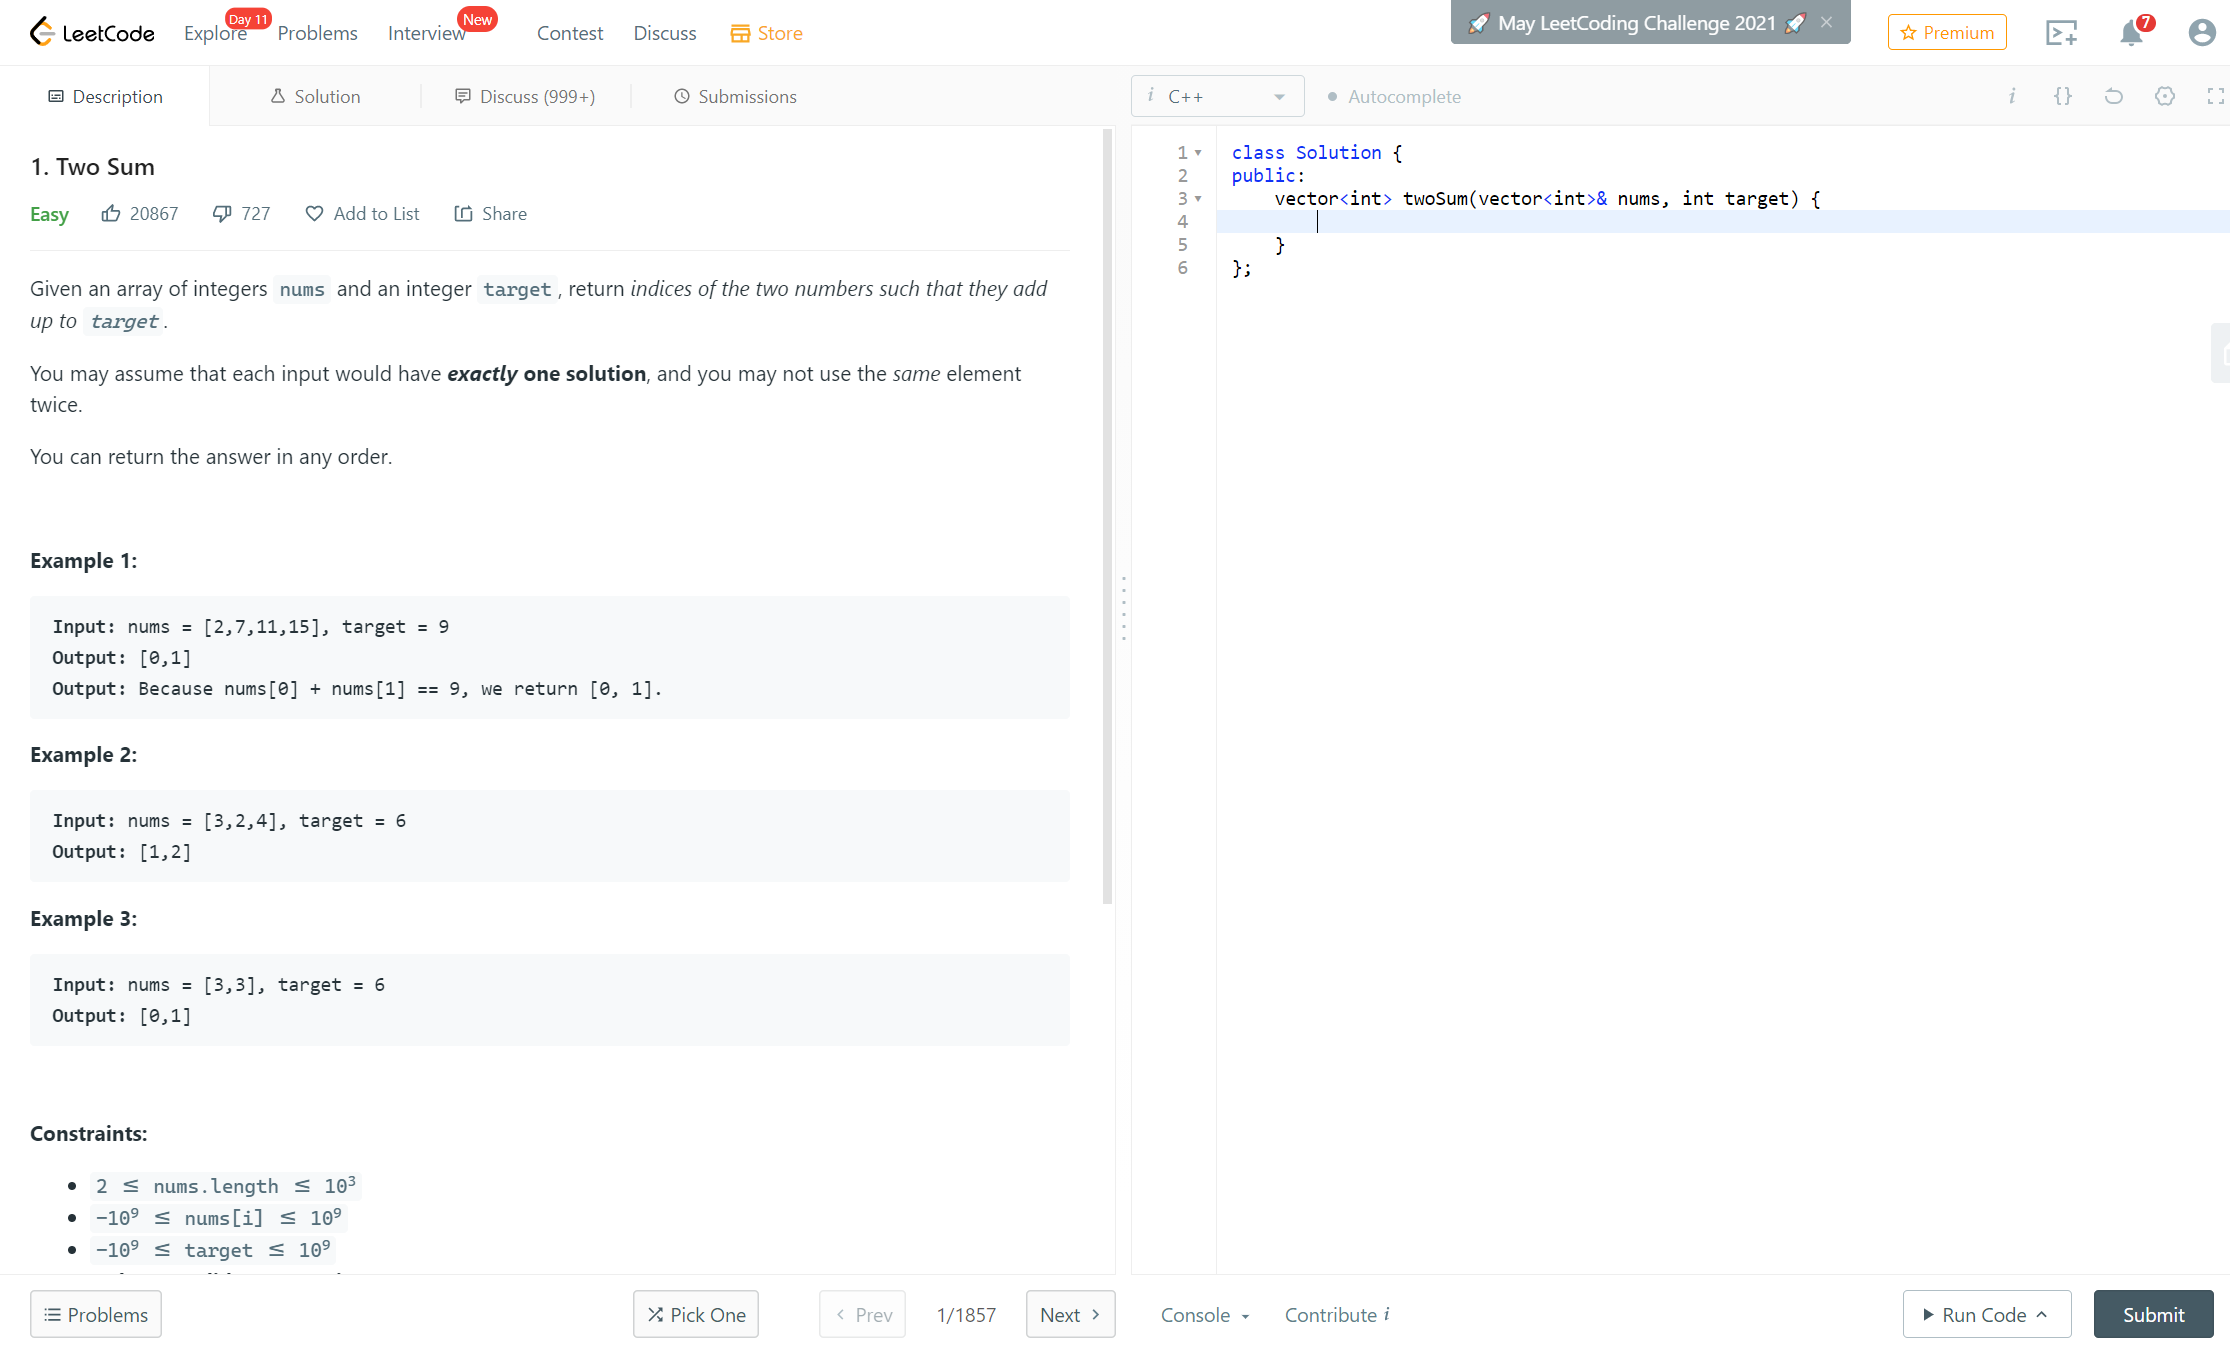
\includegraphics[width=\linewidth]{Two-Sum-LeetCode-Coding}

This is the main coding area of LeetCode. The question is on the left and the code editor is on the right, the user can write their code in the code editor and submit their solutions by clicking the button at the down right corner. This layout is a good design as the question and the code editor are displayed on the same screen, which makes it very convenient for the user to read the question and write the code solution. User can \emph{run code} to check their solution against sample test cases in order to avoid stupid errors before formal submission for judging.

\subsubsection{Submissions}

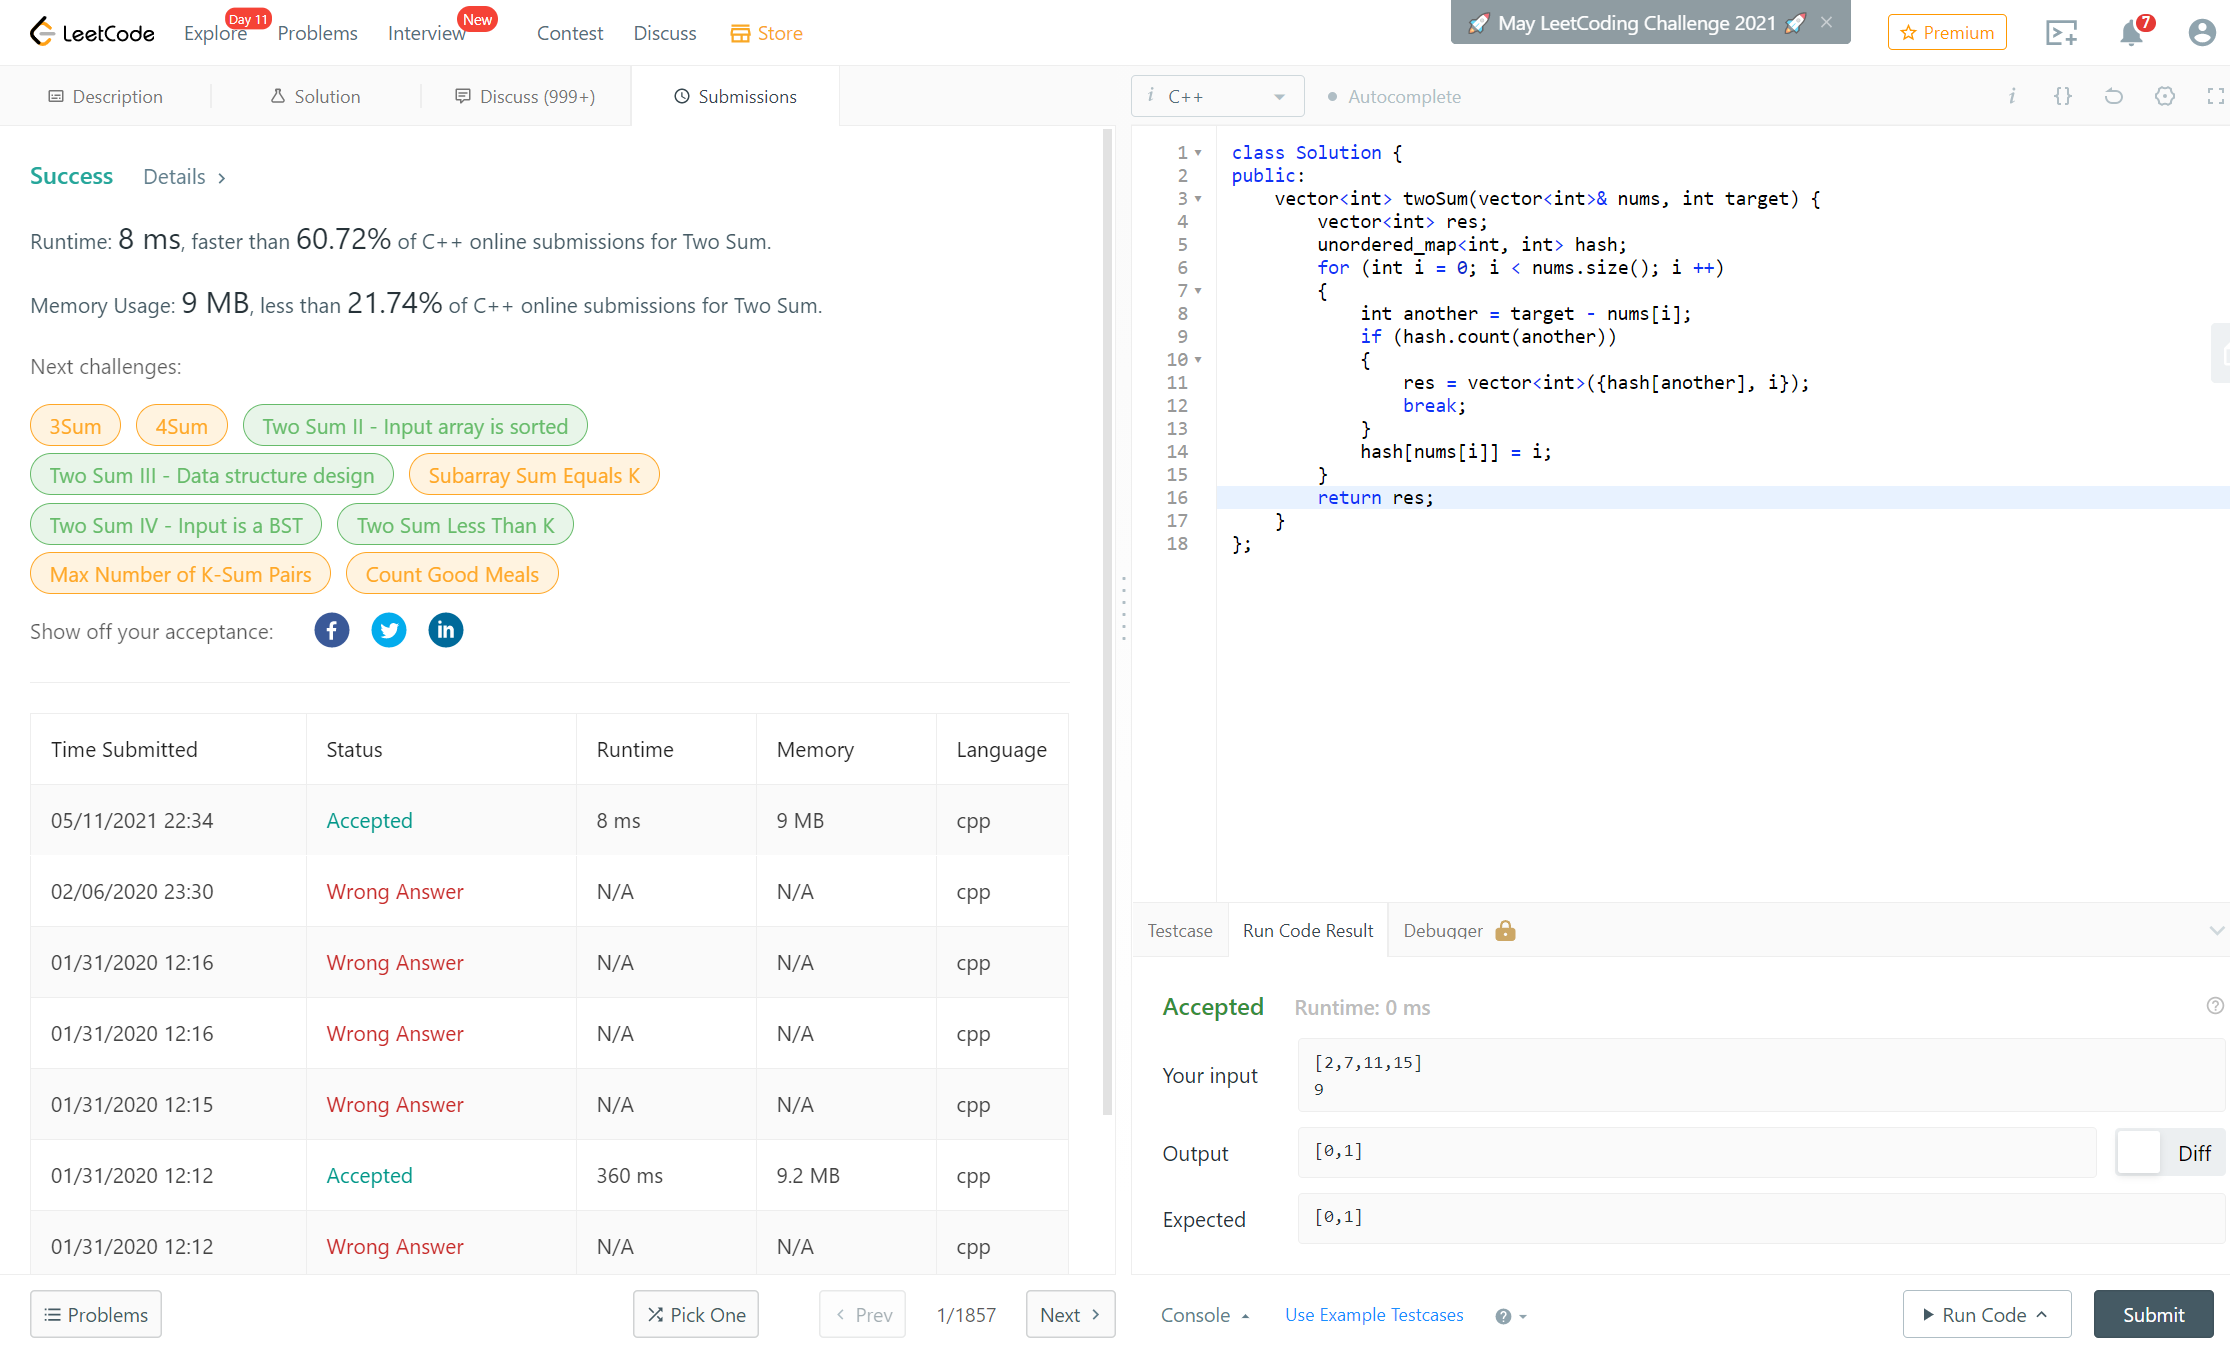
\includegraphics[width=\linewidth]{Two-Sum-LeetCode-Submission}

The submission layout displays the running time and memory usage of the user's code solution. It also compares the result with all other submissions. It lists all history submissions down below. Being able to see the stats of the submission is an interesting feature for the user.

\subsubsection{Discussion}

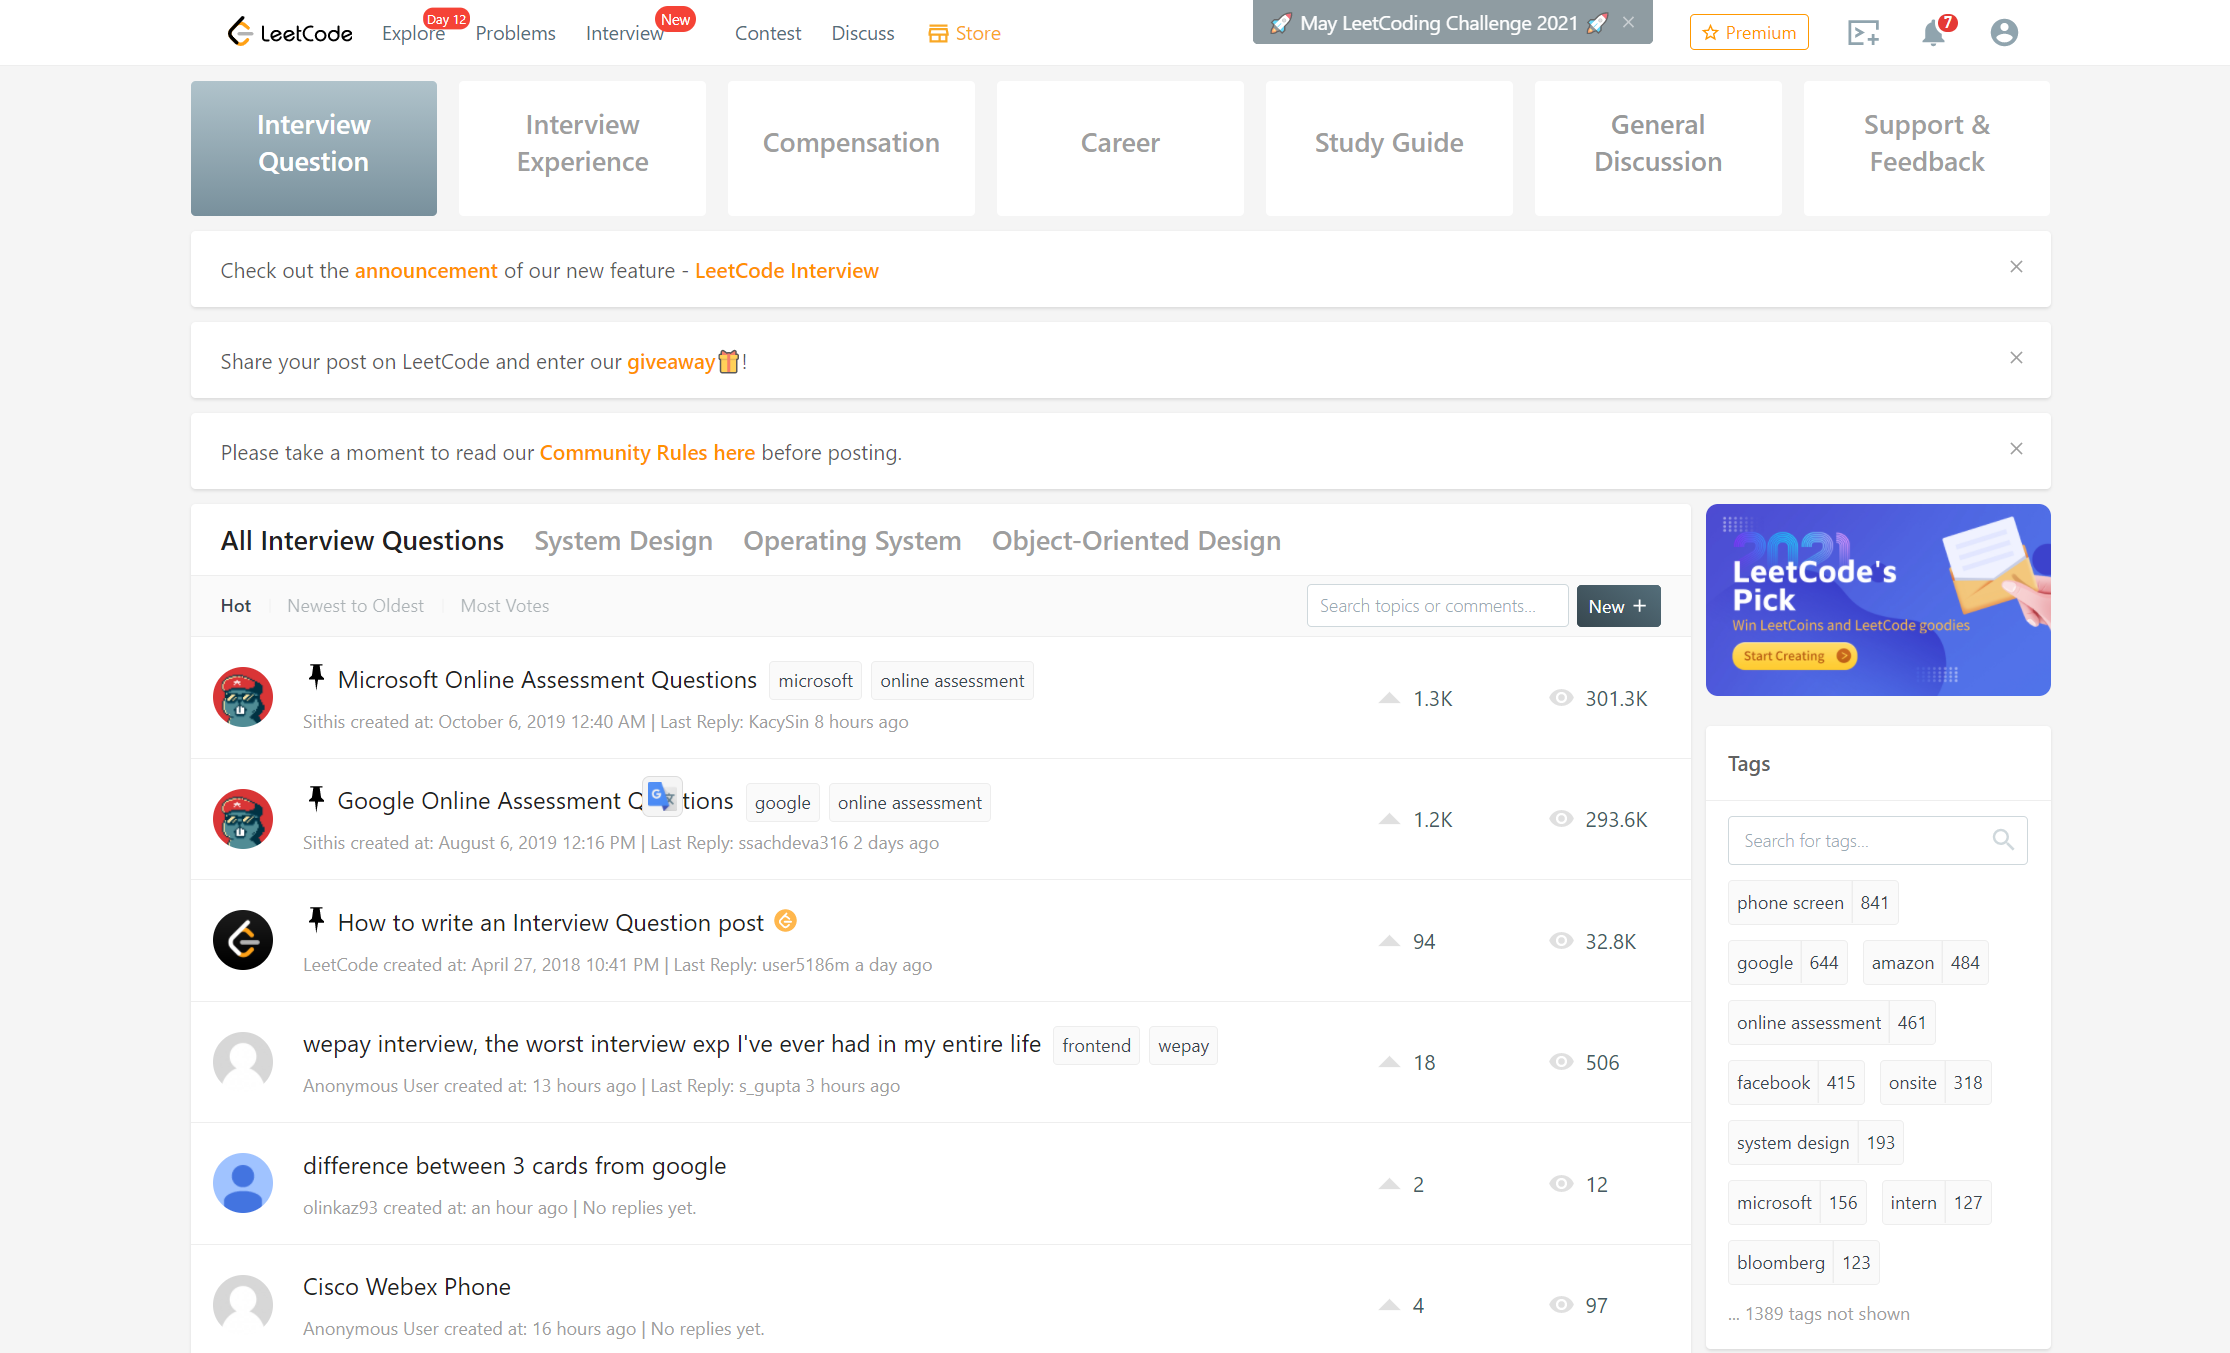
\includegraphics[width=\linewidth]{nterview-Question-LeetCode-Discuss}

There is a discussion page in LeetCode for all users to discuss the questions and their job interview experience. A good discussion environment is very helpful for self-taught programming.

\subsubsection{Contest}

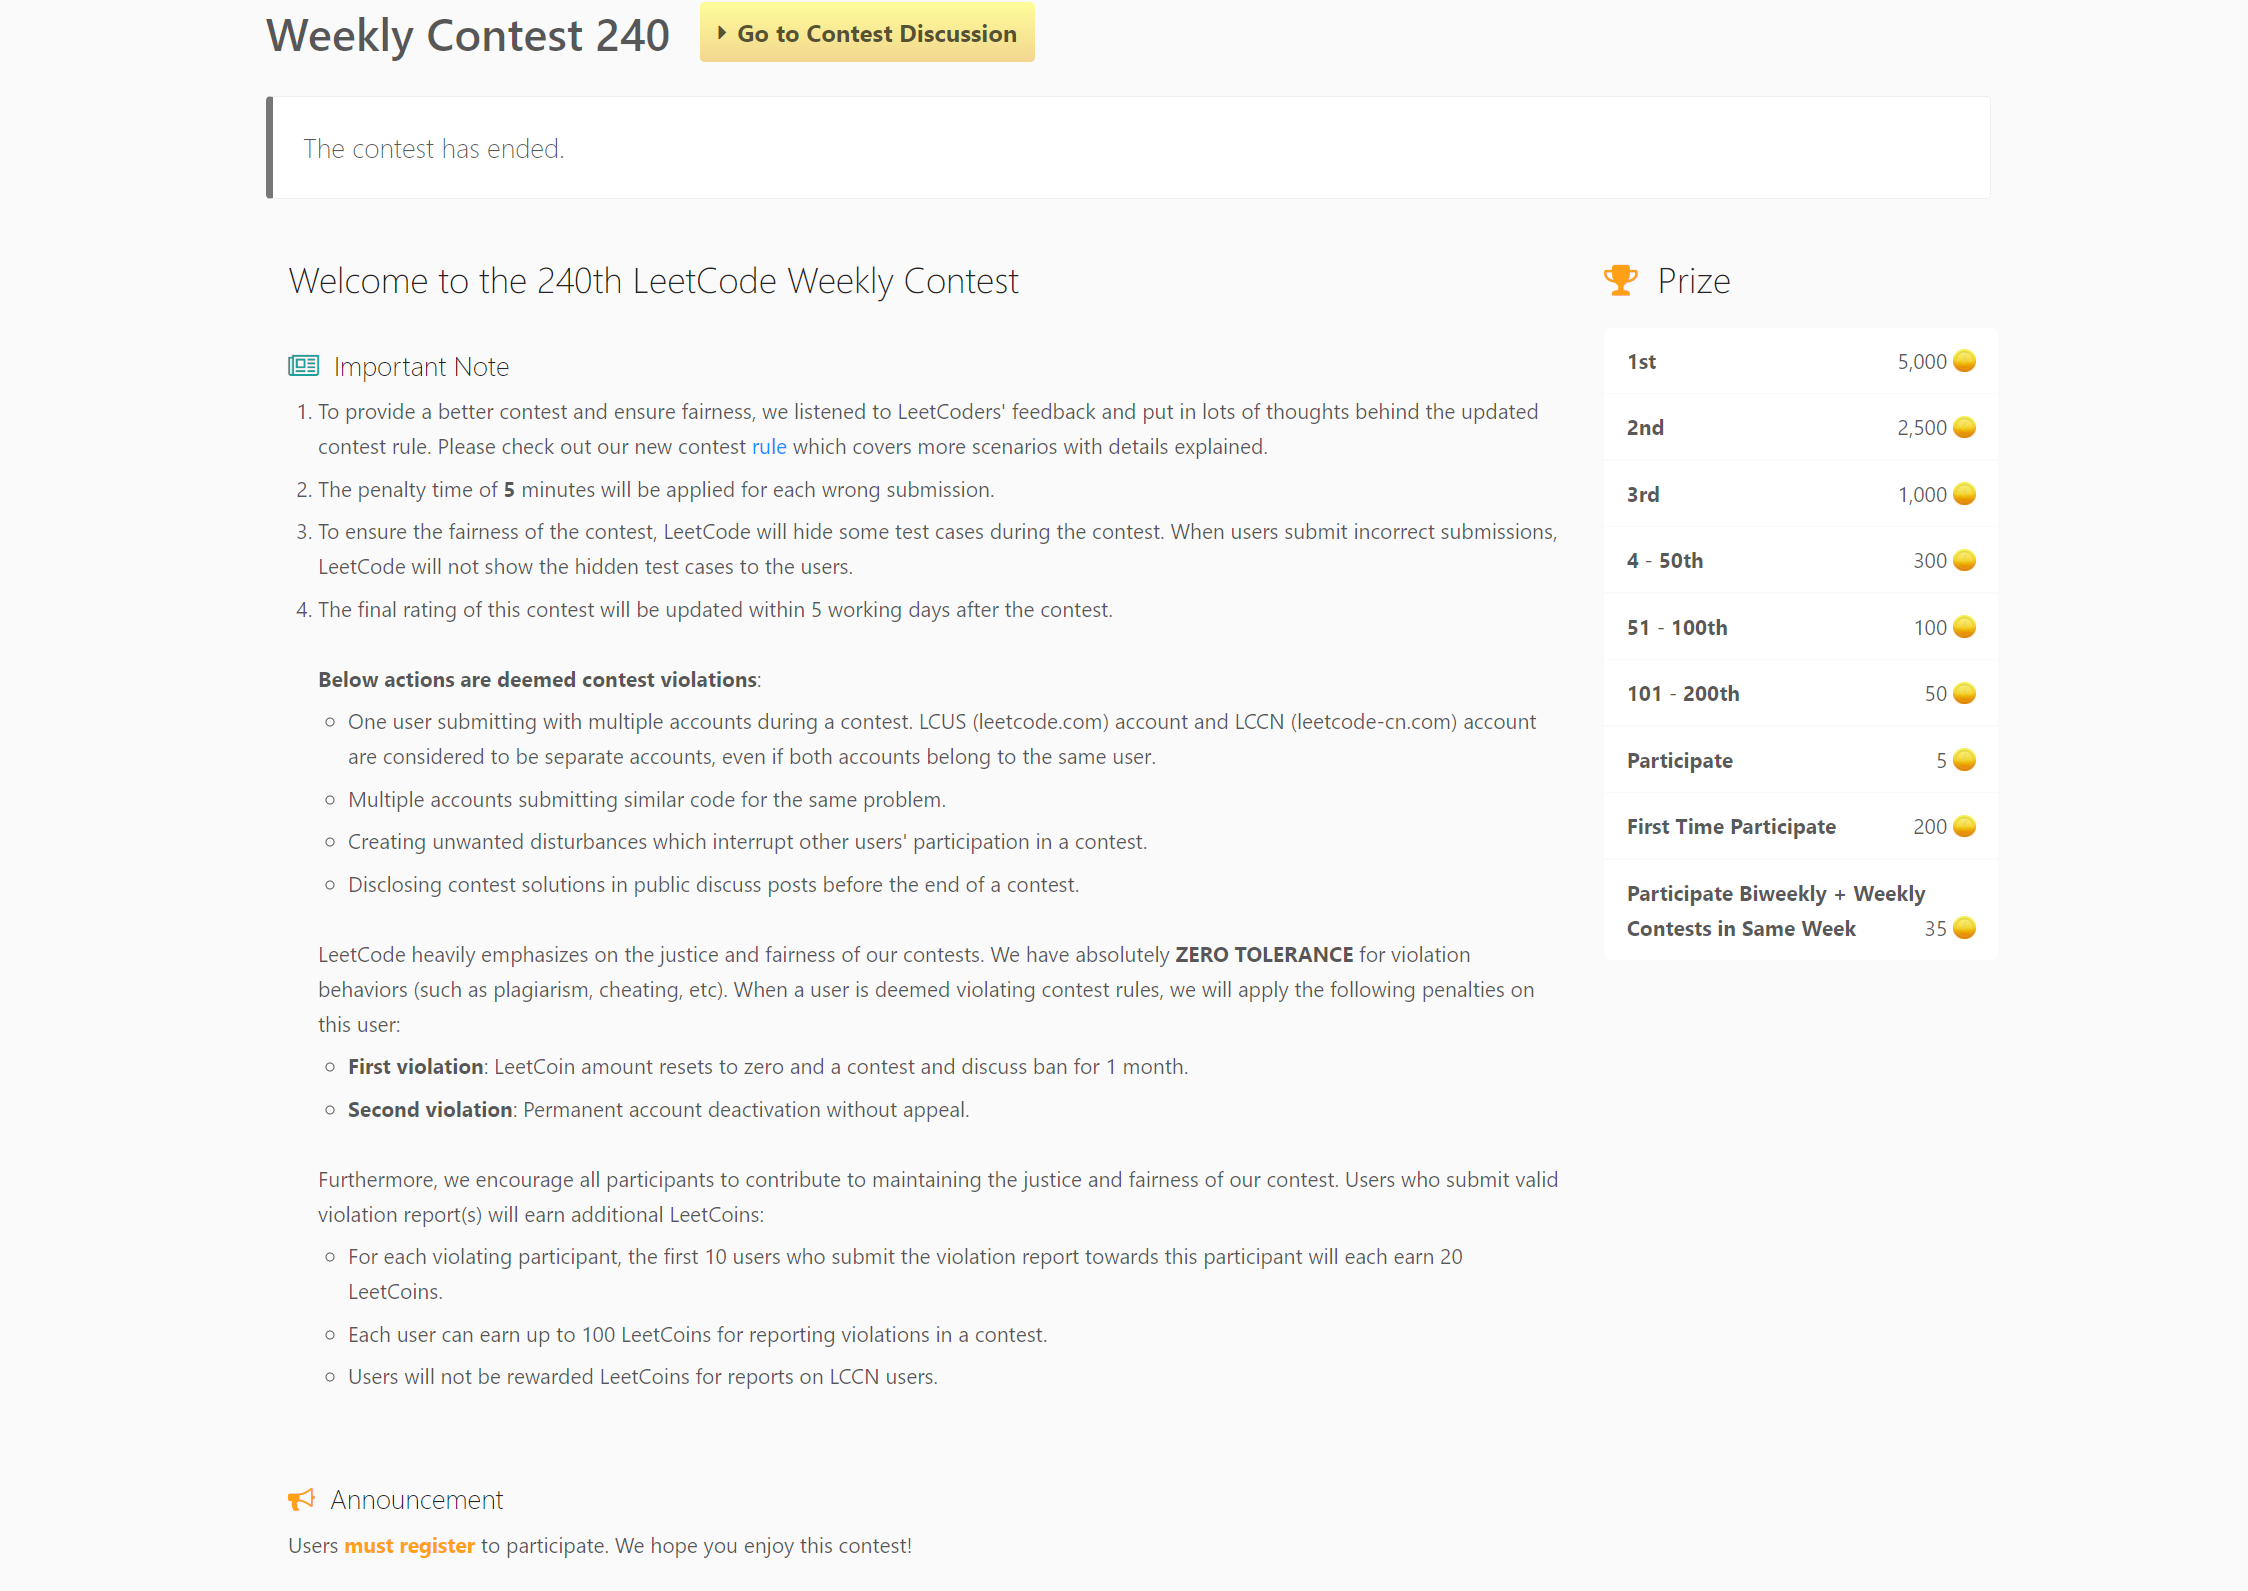
\includegraphics[width=\linewidth]{Contest-LeetCode}

LeetCode helds a contest every week, people try to solve the coding questions as quickly as possible. This motivate people's passion of learning and practicing algorithms.

\subsubsection{Pricing}


\includegraphics[width=\linewidth]{LeetCode-Premium}

The basic functions of LeetCode is free to use for all users and it charges a fee for premium subscriptions. The premium subscription provides a larger question database, better code editor, faster judger and more.

\subsubsection{Analysis}

\paragraph{Advantage}

\begin{itemize}
    \item LeetCode is fully web-based, so it works on any platform.
    \item LeetCode makes it easy to share questions and discuss them with other users.
    \item LeetCode has a clean and easy to use graphical interface.
\end{itemize}

\paragraph{Downside}

\begin{itemize}
    \item LeetCode does not allow users to create custom questions.
    \item There is no way for a teacher or a tutor to assign coursework and get statistics data.
    \item LeetCode charges a subscription fee for some essential functions.
    \item LeetCode requires a stable Internet connection to run and debug code.
\end{itemize}

\paragraph{Ideas}

\begin{itemize}
    \item The layout of the coding area is good practice.
    \item The way LeetCode organizes its question database (Tagging each question with question type/difficulty/accept rate) is good practice.
    \item My software will be completely free and open sourced with a good editor and fast judger out of the box.
    \item The \emph{run code} function for debugging before formal submission is a very useful feature.
    \item Some format of coding competition can be held by the user.
\end{itemize}

\subsection{Codeforces}

Codeforces is a competitive coding platform, it is mainly used by people to held coding competition. It takes a similar approach to judge code with test data. There is no code editor provided, user are required to write and debug their solution on their own IDE and only submit the source code for judging.

\subsubsection{Main question layout}

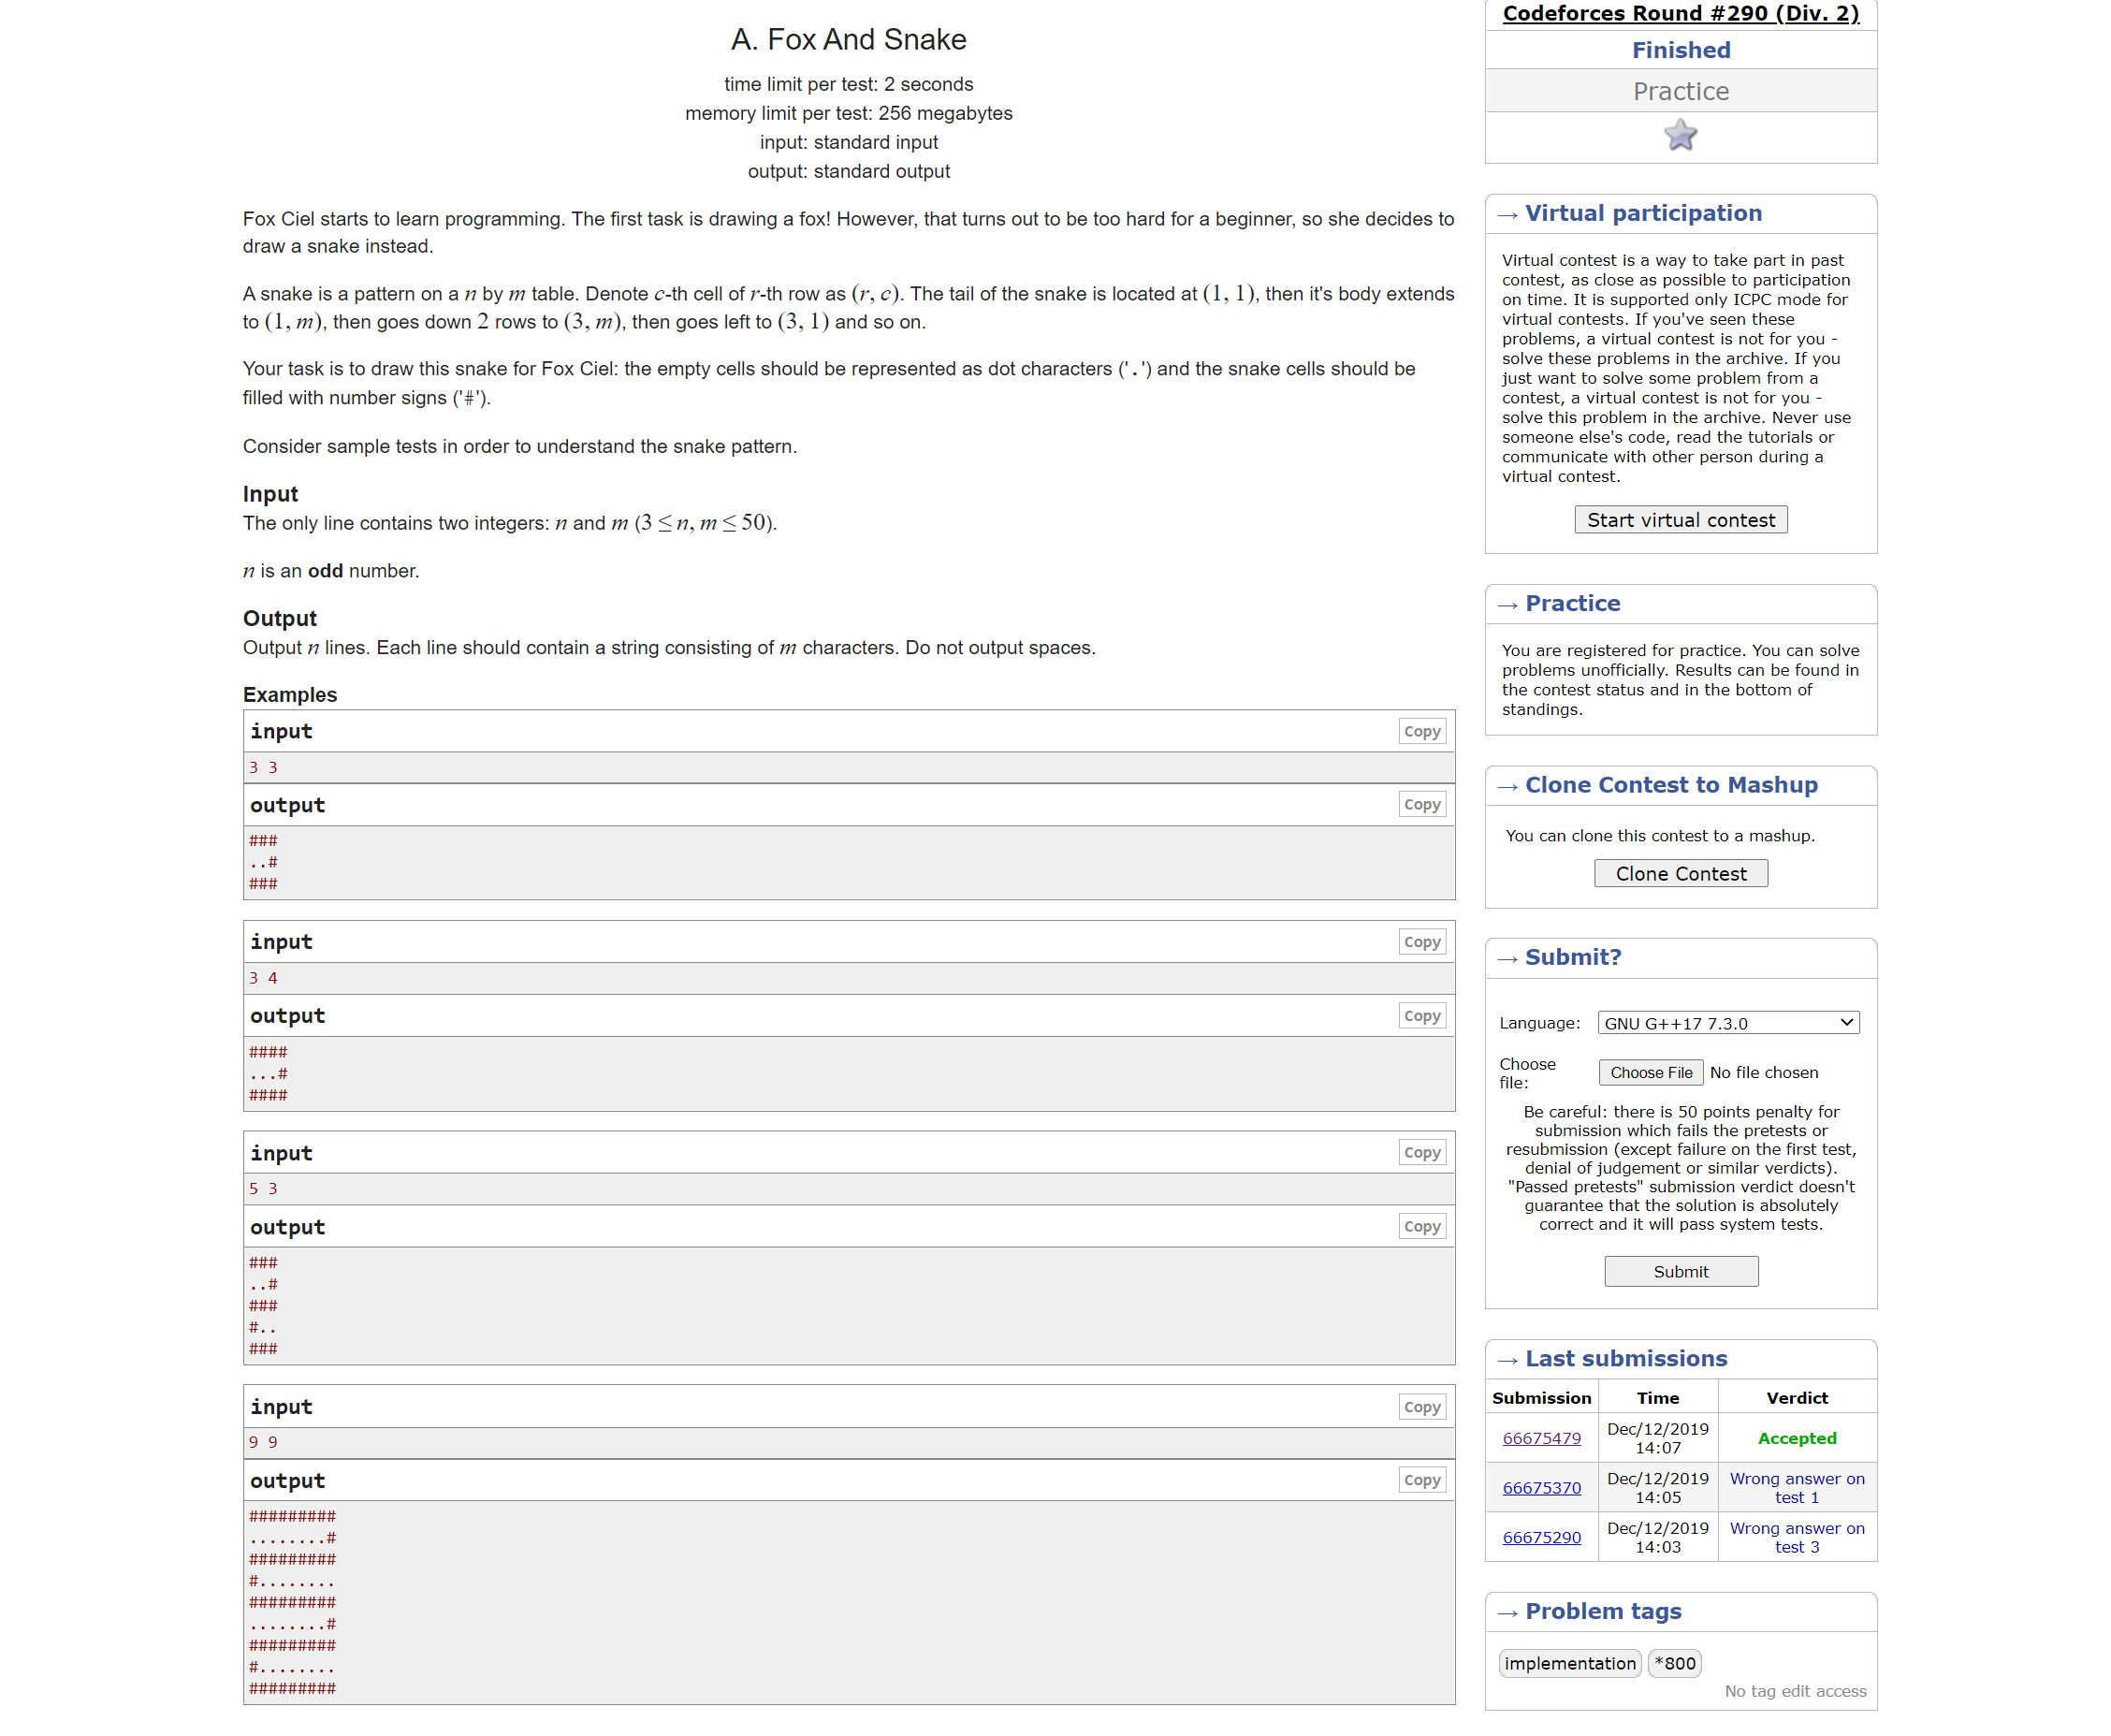
\includegraphics[width=\linewidth]{Problem-A-Codeforces}

The question layout displays the description of the question and provides sample test cases. It also shows the performance requirement for the code solution.

\subsubsection{Submission}

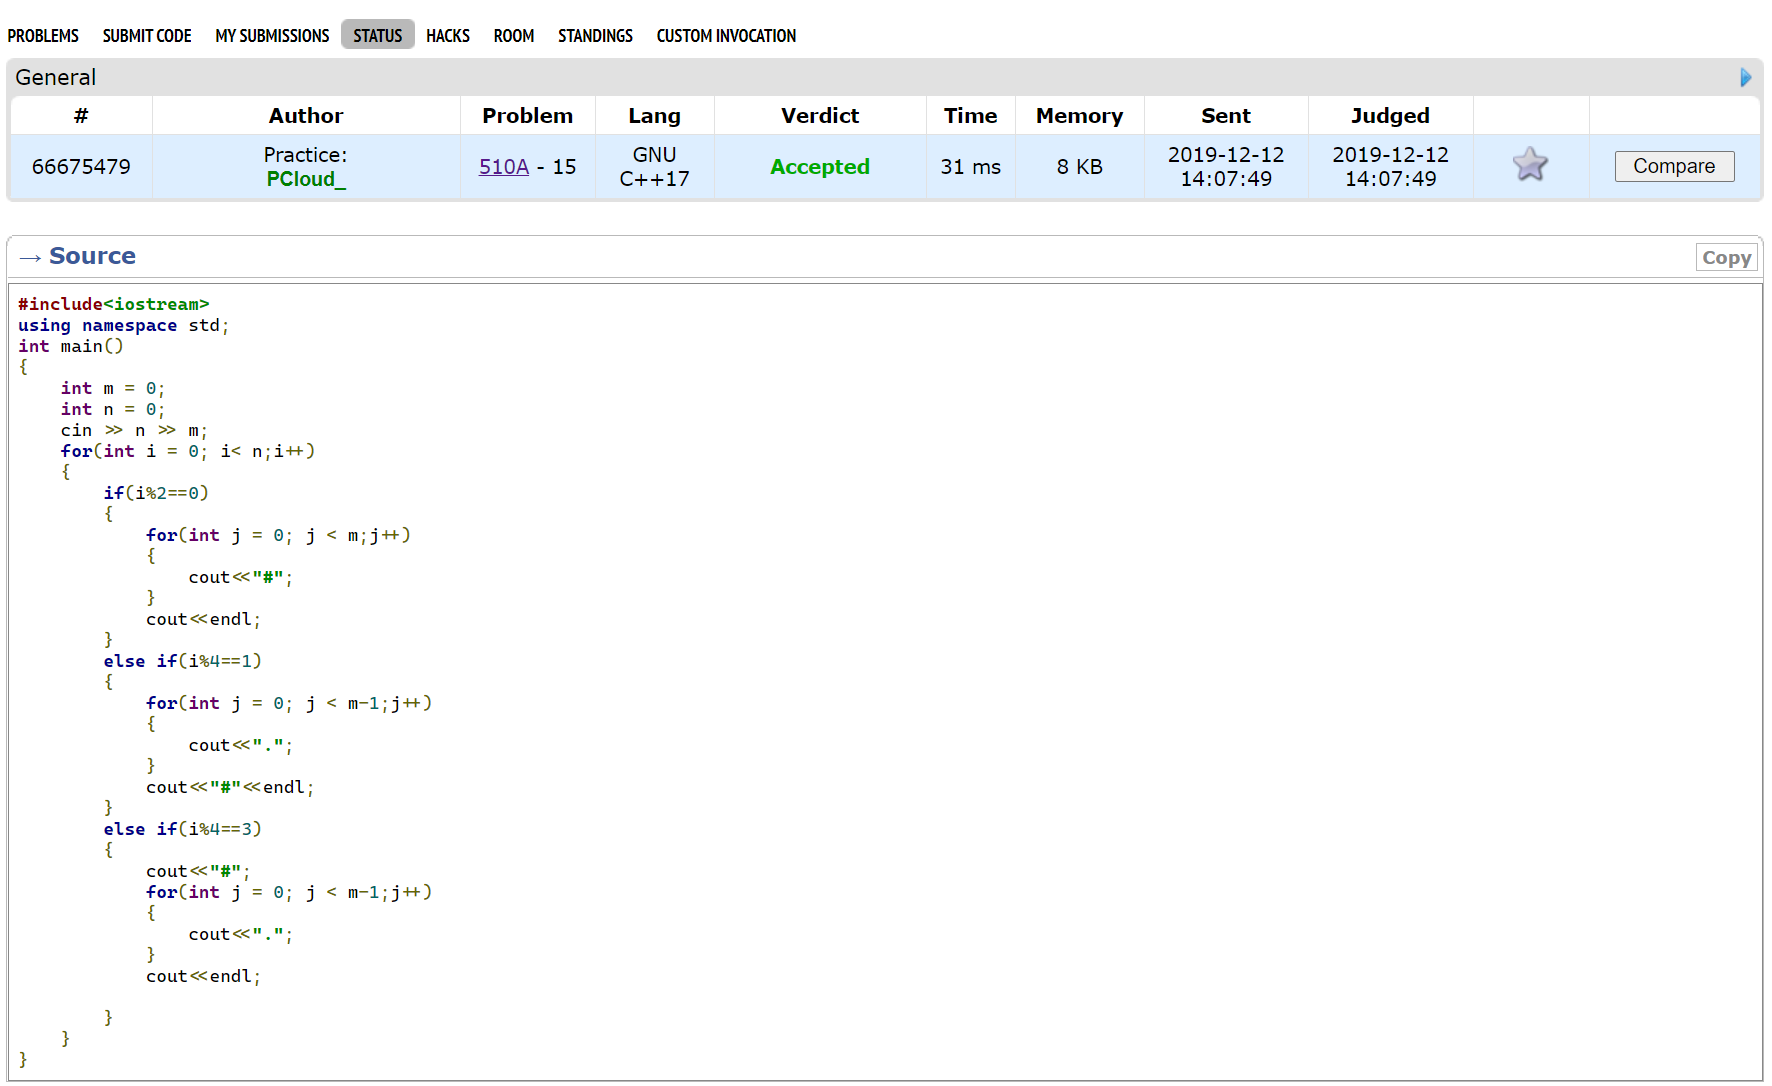
\includegraphics[width=\linewidth]{Submission-66675479-Codeforces}

When the user submits the code, the code enters a queue waiting for judging, then the user can look up their result.

\subsubsection{Contest}

Codeforces helds contest regularly similarly to LeetCode, but with much harder quesitons.

\subsubsection{Analysis}

\paragraph{Advantage}

\begin{itemize}
    \item Codeforces is completely free and it is maintained by its community.
    \item Codeforces is fully web-based so it works on any platform.
    \item Codeforces supports all mainstream programming languages.
    \item Codeforces supports custom questions.
\end{itemize}

\paragraph{Downside}

\begin{itemize}
    \item Codeforces focuses more on coding competition purpose instead of learning and practicing.
    \item Codeforces does not provide out of box code editor. Users need to write code in their own code editor.
    \item Codeforces does not provide debugging feature, users need to run and debug their code in their own runtime environment.
    \item The juding process will be very slow when many users are submitting solutions at the same time.
\end{itemize}

\paragraph{Ideas}

\begin{itemize}
    \item The sample test cases are very useful for the user to debug their code solution.
    \item Set a time and space limit for judging to prevent malicious code from using up all system resources.
    \item Provide out of box code editor, runtime environment to make the software easy to use.
    \item Use a local judger to judge the user's solution instead of uploading it to a server to speed up the judging speed. 
\end{itemize}

\section{Features}

(TODO)

\begin{center}
\begin{tabular}{ |c|c|c| } 
 \hline
 cell1 & cell2 & cell3 \\ 
  \hline
 cell4 & cell5 & cell6 \\ 
  \hline
 cell7 & cell8 & cell9 \\ 
 \hline
\end{tabular}
\end{center}

\section{Limitations}

There are a few limitations of this software.

The software is written in Python instead of web-based which means extra software needs to be downloaded by the user. Because Python has good cross-platform compatibility, the software can still run on all mainstream platform (Windows, Mac OS and Linux) which minimize the inconvenience, but downloading an extra software is still inconvenient and may violate the IT security policy of some schools.

The judger can only accept code submission in Python. The reason for choosing Python is because it has a very similar grammar to the pseudocode and most students are already very familiar with it. Creating a compiler for `Pseudocode Programming Language' is too complex for this project. So only Python is supported for now. The reason for not supporting other programming language is that an extra runtime environment needs to be installed (compiler/interpreter), so it is not possible to support them out of the box. But some extra configuration might be provided to allow submit code solution in other languages.

Unlike LeetCode, there is no Discussion pages for users to discuss questions because it is a Python program instead of a web one. But this is not a big problem, students and teachers should use an existing product such as Microsoft Teams which has very good support in sharing code snippets. It is unnecessary to rebuild the wheel.

Distribute the questions and assignments is still something inconvenient. Currently, distributing questions and assignments requires the teacher to first export the questions and assignments, then send them to the students through email or file-sharing platforms. When the students finish working, they need to send their result back through email or other apps. I have attempted to integrate the file-sharing function with the existing platform - the Microsoft Teams Assignment function. But very, unfortunately, the Graph API required for this operation is still in beta version, which means it can only be tested in the development environment and cannot be used in production. So for now, the users still have to use this inconvenient way to share questions and submissions. But the further, the integration with some existing platforms may improve the experience.

There are no good ways to maintain and distribute a large question database. Computer Science teachers are requied to maintain a database for their own students. But this is a difficult work. Creating good test cases is much time consuming than writing a mark scheme, it is very likely for a wrong solution to pass the judging if the test cases are not good enough. It relies on the teacher who creates the questions to consider everything clearly to minimize its impact.

The judger can only simply compare the students' output with the expected output, if there is a format error such as trailing space and extra newline in their output, which will not be considered as a mistake in a real exam, will be marked as a wrong answer by the judger. So students may need to spend extra time debugging their output format.

\section{Hardware and software requirements}

Due to the good compatibility of Python, it can run on all mainstream desktop operating systems. Linux, macOS and Windows. The software itself does not contain complex graphical effects or large scale computation. So it should be able to run under 1C CPU and 512M RAM. However, the code solutions provided by the students may need more resource to run and test. So 2C CPU and 2G RAM is recommended.

(TODO)

\begin{center}
    \begin{tabular}{ |c|c|c| }
        \hline
        cell1 & cell2 & cell3 \\
        \hline
        cell4 & cell5 & cell6 \\
        \hline
        cell7 & cell8 & cell9 \\
        \hline
    \end{tabular}
\end{center}

\section{Success criteria}

(TODO)

\begin{center}
    \begin{tabular}{ |c|c|c| }
        \hline
        cell1 & cell2 & cell3 \\
        \hline
        cell4 & cell5 & cell6 \\
        \hline
        cell7 & cell8 & cell9 \\
        \hline
    \end{tabular}
\end{center}


\chapter{Design}

This is the design chapter.

(TODO)

Sample flow chart

\tikzstyle{startstop} = [rectangle, rounded corners, minimum width=3cm, minimum height=1cm,text centered, draw=black, fill=red!30]
\tikzstyle{io} = [trapezium, trapezium left angle=70, trapezium right angle=110, minimum width=3cm, minimum height=1cm, text centered, draw=black, fill=blue!30]
\tikzstyle{process} = [rectangle, minimum width=3cm, minimum height=1cm, text centered, draw=black, fill=orange!30]
\tikzstyle{decision} = [diamond, minimum width=3cm, minimum height=1cm, text centered, draw=black, fill=green!30]
\tikzstyle{arrow} = [thick,->,>=stealth]

\begin{tikzpicture}[node distance=2cm]
    \node (start) [startstop] {Start};
    \node (in1) [io, below of=start] {Input};
    \node (pro1) [process, below of=in1] {Process 1};
    \node (dec1) [decision, below of=pro1, yshift=-0.5cm] {Decision 1};
    \node (pro2a) [process, below of=dec1, yshift=-0.5cm] {Process 2a};
    \node (pro2b) [process, right of=dec1, xshift=2cm] {Process 2b};
    \node (out1) [io, below of=pro2a] {Output};
    \node (stop) [startstop, below of=out1] {Stop};
    \draw [arrow] (start) -- (in1);
    \draw [arrow] (in1) -- (pro1);
    \draw [arrow] (pro1) -- (dec1);
    \draw [arrow] (dec1) -- node {yes} (pro2a);
    \draw [arrow] (dec1) -- node {no} (pro2b);
    \draw [arrow] (pro2b) |- (pro1);
    \draw [arrow] (pro2a) -- (out1);
    \draw [arrow] (out1) -- (stop);
\end{tikzpicture}

\chapter{Development}

\section{Preparation}

\subsection{Code editor}

Download and install \href{https://code.visualstudio.com/}{VS Code}.

Instead of using a large IDE with everything pre-configured, I decide to use a code editor to write source code and a terminal to execute commands. This gives me more control on my project.

VS Code is a free and open source code editor which also have greate support for Python.

I decide to use VS Code as my code editor.

\subsection{Runtime environment}

Download and install \href{https://www.python.org/downloads/}{Python 3.9.5}.

I simply choose the latest Python release for this project. When I release the software, the Python interpreter will be packed with the binary files so there is no need to worry about the compatibility with the Python installation in users' environment.

\subsection{Version control}

Download and install \href{https://git-scm.com/}{Git}.

Git is a free and open source distributed version control system. It records every \emph{commit} I made to the source code and allows me to revert back to any previous \emph{commit}. This makes it easy to roll back to a certain version and locate bugs. It also allow me to create new \emph{branches} which is useful when experimenting new features without worrying about damaging the stable code.

I decide to use Git as the version control system for this project.

\subsection{Project management}

\href{https://github.com}{GitHub} is a code hosting platform which supports many project management features. The \emph{Issue} allows my stakeholders to report bugs and suggests features easily. The \emph{Action} provides support for CI/CD. The \emph{Project} provides support for managing and organizing the TODO list for the project.

I decide to use GitHub as the code hosting platform for this project.

\subsection{Create a project repository}

I need to create a private repository to store and manage the source code.

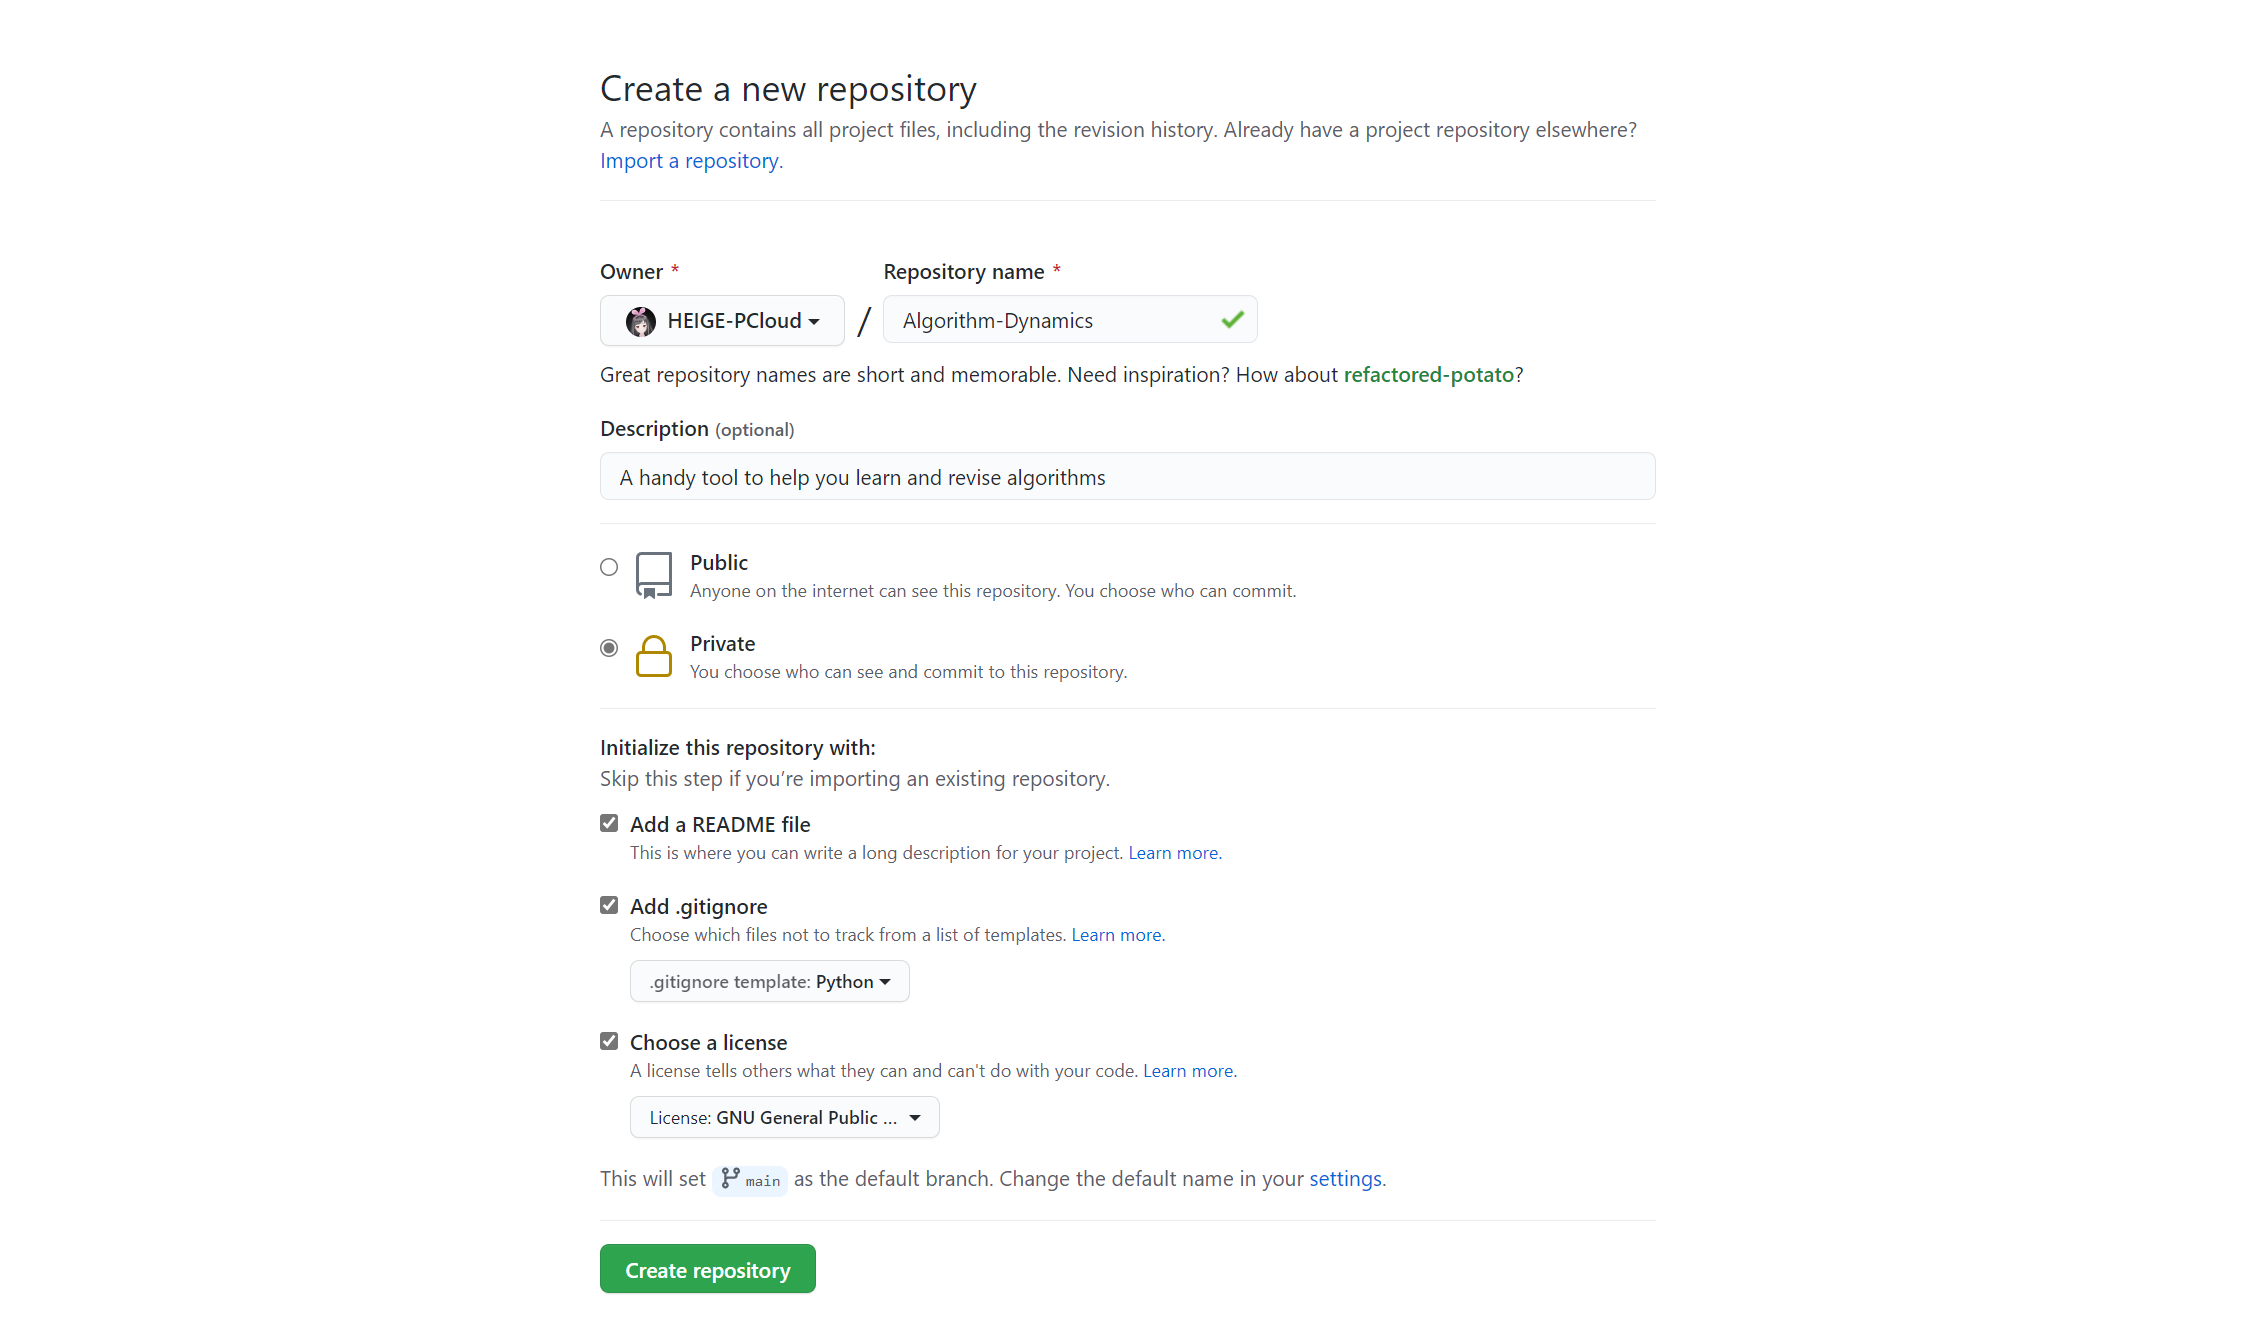
\includegraphics[width=\linewidth]{Create-a-New-Repository}

This is the inital screenshot of this project repository, there is not many things there right now, but it will be much more vivid as time goes forward.

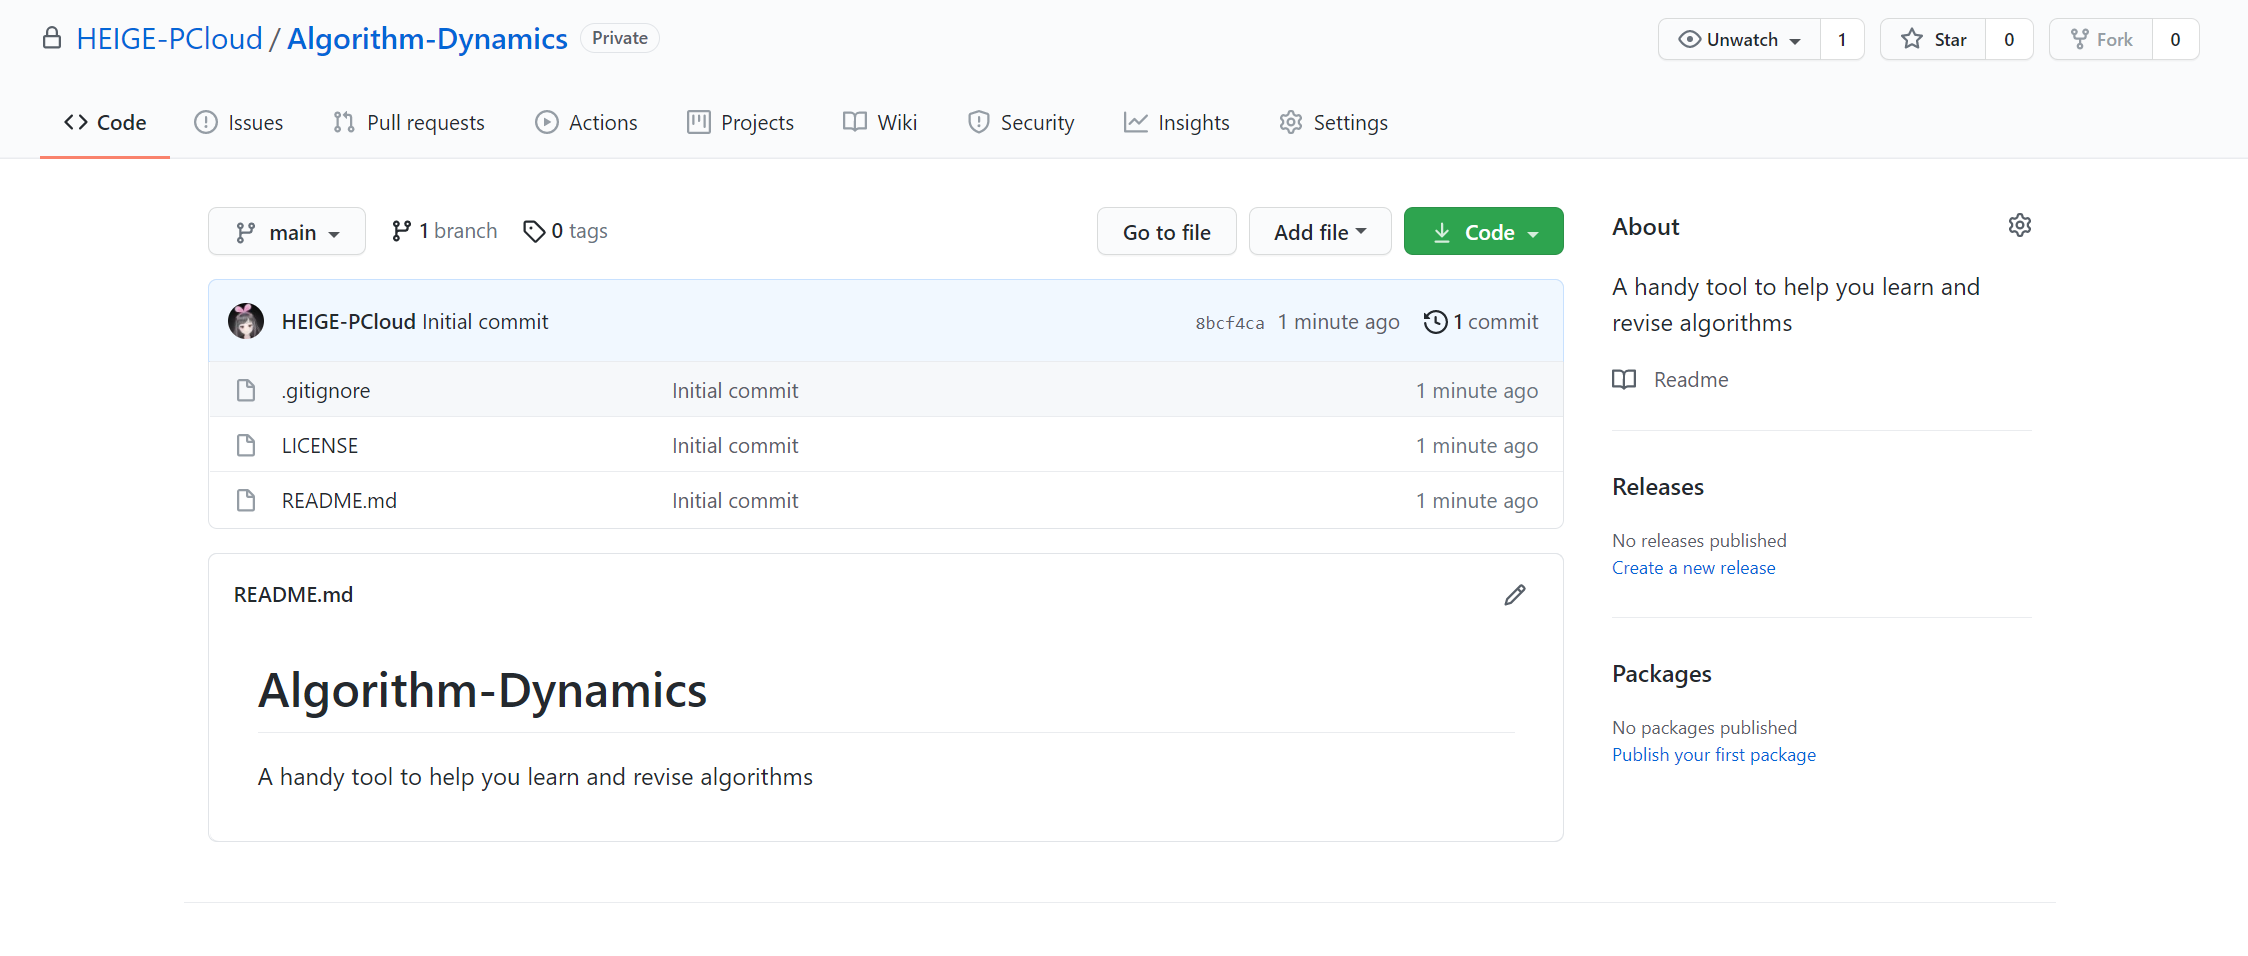
\includegraphics[width=\linewidth]{HEIGE-PCloud-Algorithm-Dynamics-A-handy-tool-to-help-you-learn-and-revise-algorithms}

I need to \mintinline{text}{clone} this repository in order to add files and write code to it.

\begin{minted}{bash}
git clone https://github.com/HEIGE-PCloud/Algorithm-Dynamics.git
cd Algorithm-Dynamics
\end{minted}

\subsection{Configure Git ignore files}

The \mintinline{text}{.gitigore} file lists files not being managed by the version control system. For example, I don't want to track the changes of the cache files or the log file.

GitHub has already generated a nice \mintinline{text}{.gitigore} file for this Python project, but I need to further ignore aditional two files, the config file from the VS Code and the pdf preview of this report.

\subsection{Create the first commit}

After I have made the changes, I need to create a \emph{commit} to comfirm the chagnes and let Git record it, so I can go back here again in the future if needed.

\begin{minted}{bash}
$ git add .gitignore
$ git commit -m "chore(configure-environment): update .gitignore
- Ignore config files for VS Code
- Ignore pdf files for the report"
$ git push
\end{minted}

Now, I have created the first commit and pushed it to the remote repository.

\subsection{Create a virtual environment}

A virtual environment is a self-contained directory tree that contains a Python installation for a particular version of Python, plus a number of additional packages.

My Python program will use many external libraries, at the same time, there are other Python projects on my computer require the same library with differnt version requirements, so I need a virtual environment to isolate the dependicies for different projects.

First, I install the lastest release of virtualenv.

\begin{minted}{bash}
$ pip install virtualenv
\end{minted}

Next, I create a new virtual environment under the project folder.

\begin{minted}{bash}
$ virtualenv env
\end{minted}

Finally, I need to activate the virtual environment.

\begin{minted}{bash}
$ ./env/Scripts/activate
\end{minted}

Now I have a clean environment to install and manage all the dependicies and packages for this project.

\section{Hello World!}

\subsection{Hello GUI application}

I will create a simple GUI application to go through all the development stages to verify the environment is ready.

I will use PyQt6 as the GUI framework. \href{https://riverbankcomputing.com/software/pyqt}{PyQt} is a set of Python bindings for The Qt Company's \href{https://www.qt.io/}{Qt application framework} and runs on all platforms supported by Qt including Windows, macOS, Linux, iOS and Android.

PyQt is licensed under \href{https://www.gnu.org/licenses/gpl-3.0.en.html}{GNU GPL v3}, which means the program needs to licensed under GNU GPL v3 as well.

Fisrt, I install PyQt6 in the virtual environment.

\begin{minted}{bash}
$ (env)  pip install PyQt6
\end{minted}

I then create \mintinline{text}{helloworld.py} under \mintinline{text}{src} folder as the source code file for the Hello World application.

In this hello world program, I will create a custom widget contains a text label and a button. The text label will display a hello world sentence. When the button is clicked by the user, the text will randomly change to the hello world message in another language.

\inputminted{python}{../src/helloworld.py}

I run the GUI Application with the following command.

\begin{minted}{bash}
$ (env) pythonw ./src/helloworld.py
\end{minted}

An hello world window shows up correctly. When the I click the  button, the text in the middle will change randomly.

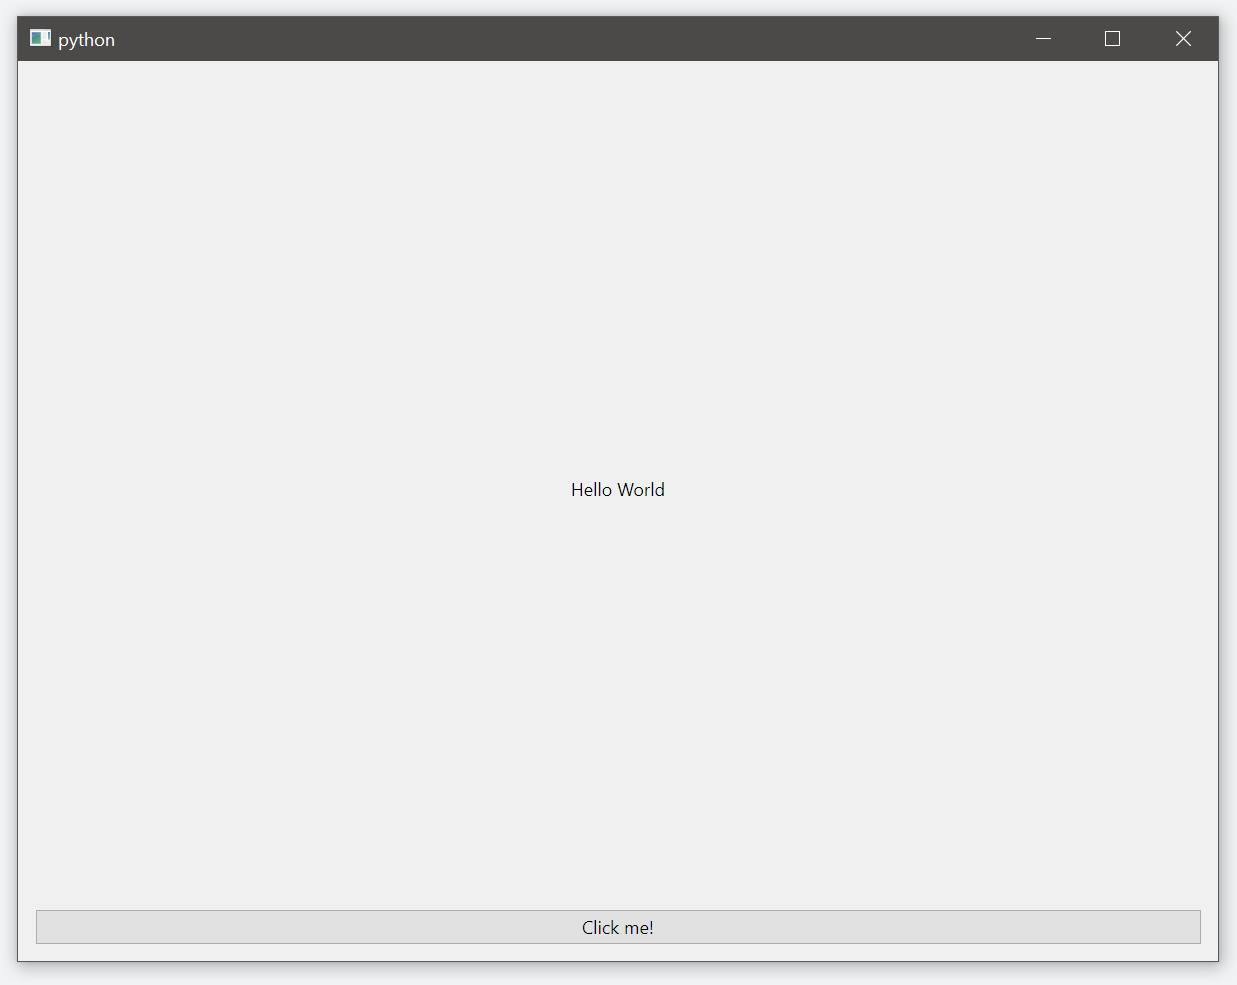
\includegraphics[width=\linewidth]{Hello-World.png}

\subsection{Hello unit test}

I am going to automate the test process with \href{https://docs.pytest.org/}{Pytest} unit test framework. It can run through my pre-set test data automatically without me clicking each button or inputing each value by hand. This saves a lot of time and improves the quality of my tests.

I need to install Pytest into my virtual environment first.

\begin{minted}{bash}
$ (env) pip install Pytest
\end{minted}

Next I need to write the test code for the hello world program. Under \mintinline{text}{test} folder, I create \mintinline{text}{test_helloworld.py}.

Here I create three tests for the hello world program. First I test its initial state, this ensure the widget loads up with the correct text and layout. Second I test its \mintinline{python}{sayHello} function to make sure the text is changed correctly (white box test). Third I test its button, I simulate the click with \mintinline{python}{QTest.mouseClick} to make sure the button is working (black box test).

\inputminted{python}{../tests/test_helloworld.py}

\subsection{Hello coverage}

\emph{Coverage} is a measure used to describe the degree to which the source code of a program is executed when a test runs. A program with high test coverage has had more of its source code executed during testing, which suggests it has a lower chance of containing undetected software bugs compared to a program with low test coverage. I will use the coverage to provide evidence for the quality of my tests.

I need to install Pytest-cov to calculate the coverage of the tests.

\begin{minted}{bash}
$ (env) pip install Pytest-cov
\end{minted}

I need to add a config file for the Pytest-cov to exclude the test and debug code from the coverage calculation.

Create \mintinline{text}{.coveragerc}.

\inputminted{text}{../.coveragerc}

Now, I run the unit test with this command. \mintinline{text}{--cov} configures the folder of my source code. \mintinline{text}{--cov-report} configures the format of the coverage output, \mintinline{text}{term} lets it to be printed directly to the termial. `-vv` shows the details of my tests. \mintinline{text}{--cov-config} configures the location of our config file for coverage, which is the \mintinline{text}{.coveragerc} file I just created.

\begin{minted}{bash}
$ (env) pytest --cov=src -vv --cov-report=term --cov-config=./.coveragerc
\end{minted}

Here is the output of the test. My 3 tests \mintinline{python}{test_initWidget}, \mintinline{python}{test_sayHello}, \mintinline{python}{test_mouseClick} are executed and passed correctly. And the coverage report shows that the coverage of my tests is 100\% which means all code is executed during the tests. I aim for a 95\%+ coverage for the formal project.

\begin{minted}{text}
========================== test session starts ==========================
platform win32 -- Python 3.9.5, pytest-6.2.4, py-1.10.0, pluggy-0.13.1 --
cachedir: .pytest_cache
plugins: cov-2.12.0
collected 3 items

tests/test_helloworld.py::test_initWidget PASSED [ 33%]
tests/test_helloworld.py::test_sayHello PASSED  [ 66%]
tests/test_helloworld.py::test_mouseClick PASSED [100%]

------------ coverage: platform win32, python 3.9.5-final-0 ------------
Name                Stmts   Miss Branch BrPart  Cover
-----------------------------------------------------
src\__init__.py         0      0      0      0   100%
src\helloworld.py      17      0      0      0   100%
-----------------------------------------------------
TOTAL                  17      0      0      0   100%


=========================== 3 passed in 0.53s ===========================
\end{minted}

\subsection{Hello static check}

The style of the code is important as well. It will make the maintenance much easier if all variables have meaningful names, no trailing whitespace, proper blank lines, etc. I will use the tool flake8 to perform static check of my code. flake8 nicely works with VS Code, so I will have useful notifications so these issues can be fixed quickly.

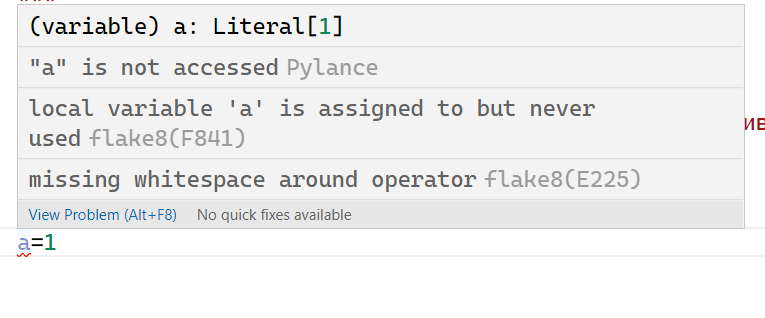
\includegraphics[width=\linewidth]{flake8.png}

Another useful tool is autopep8, it auto formats my source code and decides the whichspaces and blank lines wisely. 

I install these two tools to monitor and improve the style of my code.

\begin{minted}{bash}
$ (env) pip install flake8 autopep8
\end{minted}

\subsection{Hello requirements.txt}

I have installed a lot of packages for my project. \mintinline{text}{requirements.txt} is a file records all the packages I have installed, so the packages can be easily managed.

\begin{minted}{bash}
$ (env) pip freeze > requirements.txt
\end{minted}

\subsection{Hello CI/CD}

Continuous integration (CI) and continuous delivery (CD) embody a culture, set of operating principles, and collection of practices that enable application development teams to deliver code changes more frequently and reliably.

I will use \href{https://github.com/features/actions}{GitHub Actions} to auto test, build and deliver my application. 

I will use \href{https://codecov.io/}{Codecov} to monitor the test quailty and coverage.

Create workflow file at \mintinline{text}{.github/workflows/test-python-app.yml}.

\inputminted{yaml}{../.github/workflows/test-python-app.yml}

I can view the coverage report at Codecov.

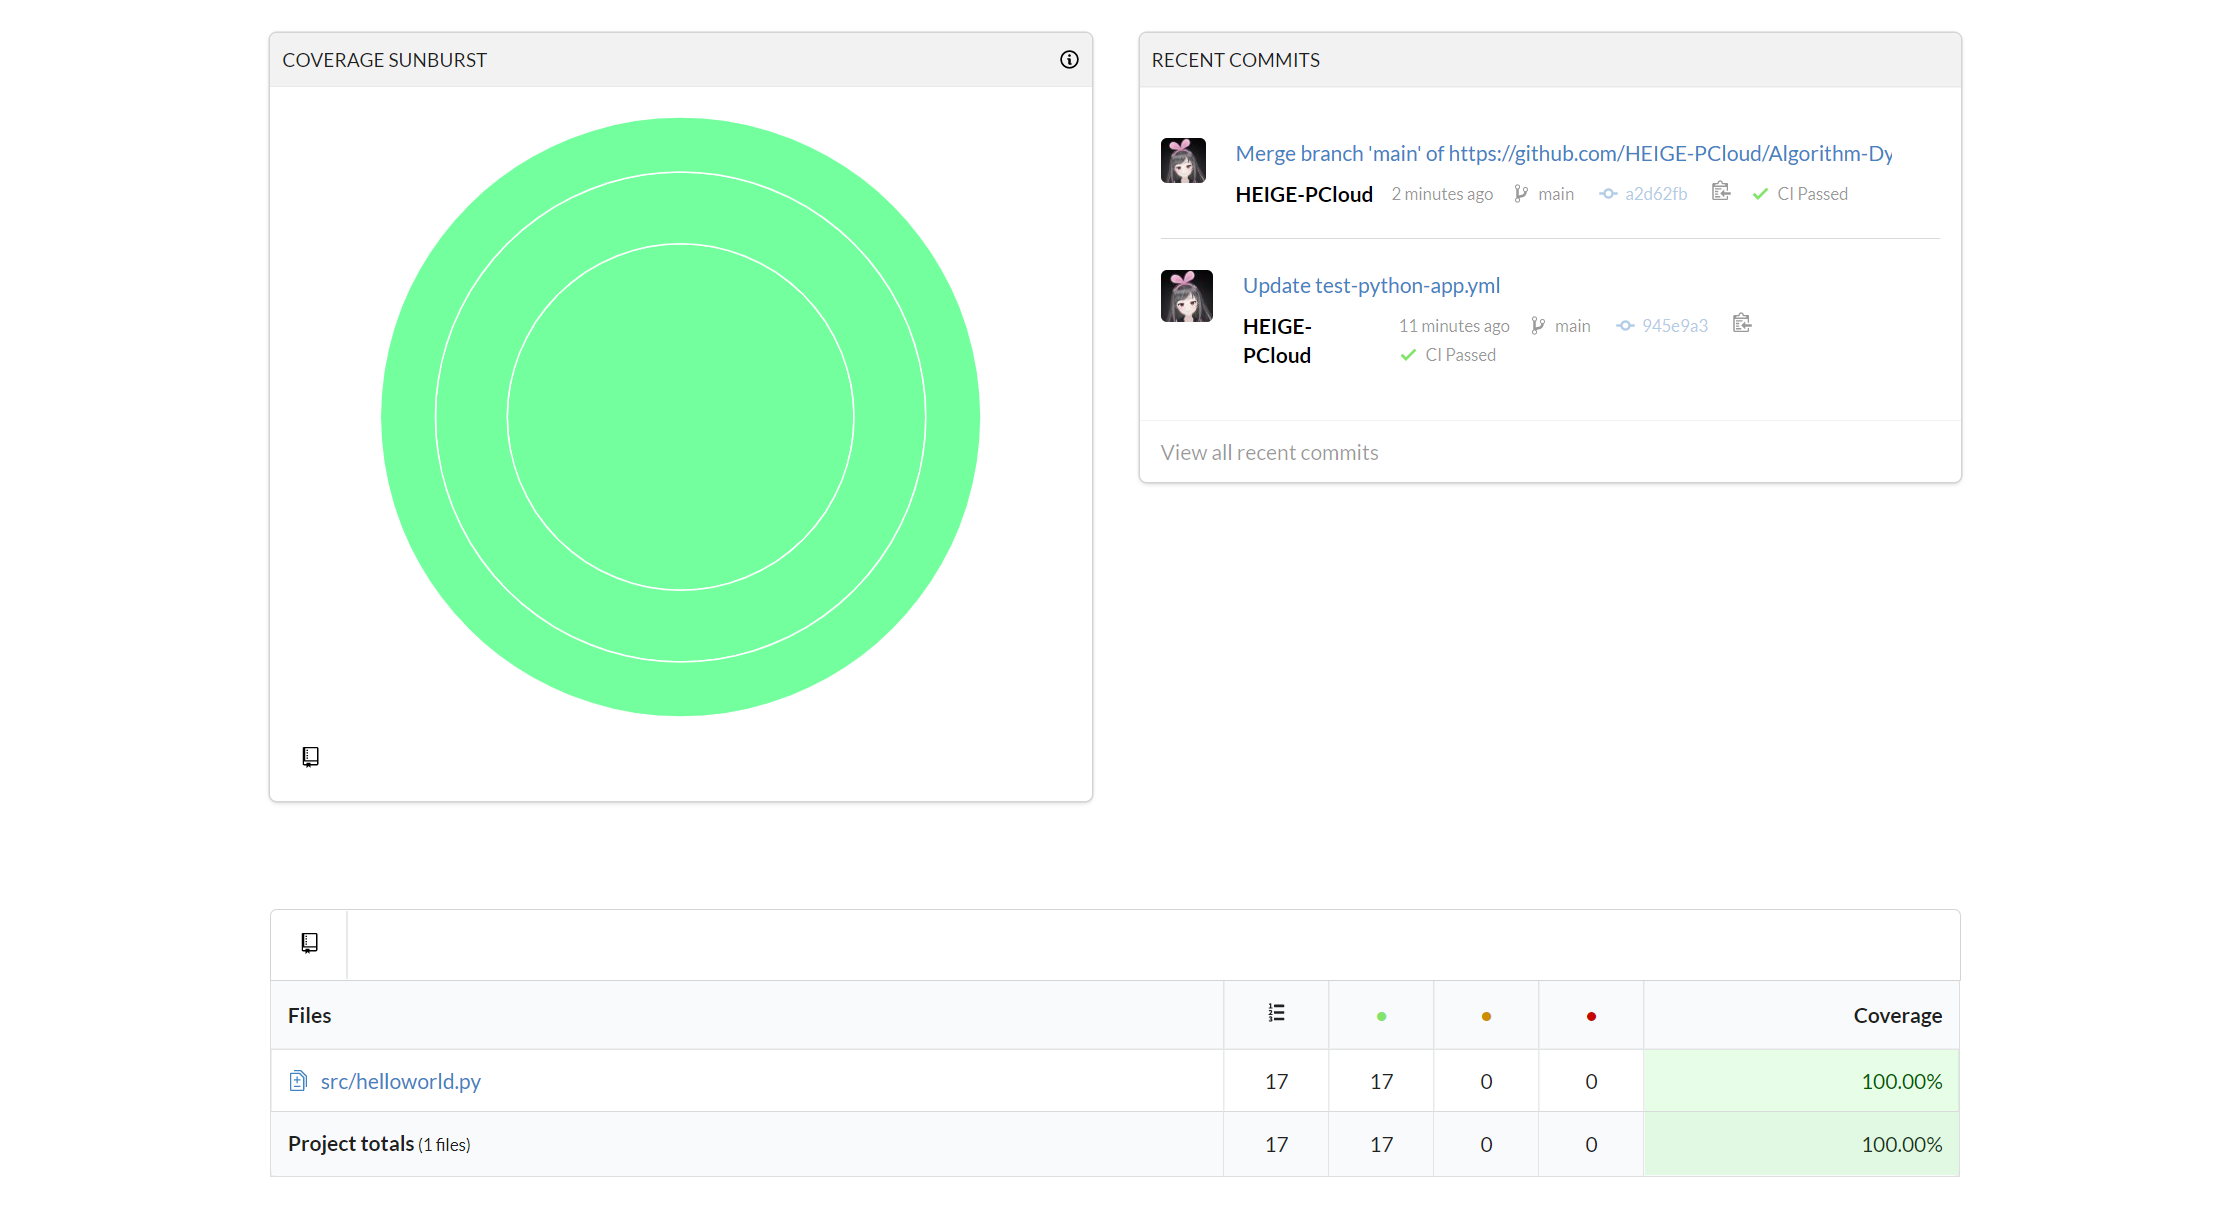
\includegraphics[width=\linewidth]{Codecov.png}

\subsection{Hello Dependabot}

The dependicies I install may get upgraded by their maintainer later during my developing process. I need them to be managed and upgraded automatically. I use GitHub Dependabot to manage the dependicies.

Configure Dependabot.

Create Dependabot config file at \mintinline{text}{.github/workflows/dependabot.yml}.

\inputminted{yaml}{../.github/dependabot.yml}

So the dependicies will be automatically checked everyday and the bot will create a new pull request when a new update is detected.

\chapter{Evaluation}

This is the Evaluation chapter.

(TODO)

\end{document}
